\documentclass[conference]{IEEEtran}

\usepackage{amsmath}
\usepackage{booktabs}
\usepackage{graphicx}
\graphicspath{{../}{../comparisons/}{../runs/}{../model_archs/arch_graph/}}
\usepackage{subcaption}
\usepackage{url}
\usepackage{array}
\usepackage{multirow}

\begin{document}

\title{Residuals Help, but Noise Rewrites the Ranking: Plant-Soil Segmentation Beyond the Clean Split}

\author{
\IEEEauthorblockN{
Junhao Bai, Changyu Chen, Xiao Dong, Jianing Liu, Alyanna Zhang
}
\IEEEauthorblockA{
\textit{School of Computer Science and Engineering} \\
University of New South Wales \\
Sydney, Australia \\
\{junhao.bai, changyu.chen1, xiao.dong, jianing.liu, alyanna.zhang\}@student.unsw.edu.au
}
}

\maketitle

\begin{abstract}
We compared traditional segmentation methods, machine learning
baselines, and deep learning models for plant-soil segmentation on the
EWS dataset. The methods include ExG, HSV thresholding, K-means,
Watershed, GrabCut, DenseCRF, Logistic Regression, Random Forest, U-Net,
ResU-Net, ASPP-ResU-Net, and Attention-Gated ASPP-ResU-Net. On the clean
test set, the deep models achieved the strongest overall performance,
with the best model reaching a Plant IoU of 0.8327, surpassing the
original paper benchmark of 0.775. Within the deep-model comparison,
the largest clean-set improvement appeared when moving from U-Net to
ResU-Net, while ASPP and attention gates provided smaller additional
gains. Even so, the traditional results showed that simple colour-based
methods such as ExG (Plant IoU 0.754) and HSV thresholding (0.708)
remained surprisingly competitive, outperforming several more complex
classical alternatives. However, the robustness results revealed a more
nuanced picture. Under strong Gaussian noise, all residual-based models
collapsed near zero Plant IoU, while the plain U-Net retained a Plant
IoU of 0.27 at the highest severity---a complete ranking reversal
relative to clean-set performance. This suggests a meaningful
accuracy-robustness trade-off: the residual-based designs that improve
clean-set accuracy in our setting also appear substantially more
vulnerable to severe Gaussian noise.
\end{abstract}

\begin{IEEEkeywords}
Plant-soil segmentation, semantic segmentation, traditional segmentation,
deep learning, robustness, domain shift, U-Net, agricultural vision.
\end{IEEEkeywords}

\section{Introduction}

Plant-soil segmentation is an important task in precision agriculture
because it supports later analysis such as crop monitoring, field
measurement, and automated decision-making. In real field scenes,
however, this task is not as simple as it first appears. Compared with
controlled laboratory images, field images are much harder to handle
because lighting changes constantly, soil appearance is often uneven,
and environmental conditions differ across time and location. As a
result, even binary segmentation can become difficult in practice.

In this project, we use the EWS Dataset released through the ETH
Research Collection~\cite{ews}. The dataset contains RGB field images
together with pixel-level masks for plant-soil segmentation. This
provides a useful setting for comparing different methods under the same
conditions. More importantly, it allows us to examine how these methods
behave not only when the images are clean, but also when the visual
conditions become less ideal.

Based on this setting, the main question of the project is
straightforward: which kinds of methods are most effective for
plant-soil segmentation in realistic field conditions? To answer this
question, we compare representative traditional segmentation methods,
machine learning baselines, and deep learning models within a unified
experimental pipeline. The traditional methods include colour- and
region-based approaches such as ExG, HSV thresholding, K-means,
Watershed, GrabCut, and DenseCRF; the machine learning baselines are
Logistic Regression and Random Forest with handcrafted features; and the
deep learning models are U-Net and its residual, multi-scale, and
attention-based variants. We evaluate all of them using the same
preprocessing and metrics, and we consider both clean-set performance
and robustness under corruption. The goal is therefore not just to
identify the best-performing model, but also to understand what actually
drives the improvement.

\section{Literature Review}

Earlier segmentation methods in agricultural vision often relied on
handcrafted rules and traditional image-processing techniques. Common
examples include vegetation indices such as Excess Green (ExG),
threshold-based segmentation, clustering, and region-based methods.
These approaches are still useful because they are easy to implement,
interpretable, and computationally cheap. However, they usually depend
heavily on stable colour contrast between vegetation and background.
Once illumination changes or the soil becomes visually complex, their
performance can drop quickly. For this reason, they are still useful as
baselines, but usually not strong enough on their own under more
difficult field conditions.

With the development of learning-based approaches, segmentation methods
gradually shifted toward models that can capture more complex visual
patterns. Traditional machine learning methods such as Logistic
Regression and Random Forest make it possible to move beyond fixed
colour rules by learning decision boundaries from handcrafted features.
In agricultural images, these features often include colour descriptors
such as RGB, HSV, and vegetation indices. Their performance is still
constrained by the quality of the input features, but they provide a
useful middle ground between hand-designed rules and fully learned deep
models.

With the further development of deep learning, segmentation methods
shifted toward representation-based models. Encoder-decoder
architectures, especially U-Net and its variants, became widely used
because they can learn pixel-level segmentation directly from data while
still preserving spatial detail through skip connections. This is
important in agricultural images, where plant regions may be small,
irregular, or visually close to the background. In these cases, the
model needs more than colour information alone; it also needs to use
local texture, boundary cues, and surrounding context.

Later studies extended this general framework in several ways. Residual
connections were introduced to improve optimization and feature reuse,
especially in deeper networks. Multi-scale modules such as ASPP were
designed to capture information at different receptive-field sizes,
while attention mechanisms were used to guide the model toward more
relevant regions and suppress background interference. Although these
ideas are different in form, they are all trying to solve a similar
problem: how to make segmentation more accurate and more reliable in
visually complicated scenes.

Recent work in plant phenotyping also shows that model performance
depends strongly on real-world variability. Deep learning methods have
already shown strong results for outdoor plant segmentation under
diverse field conditions~\cite{zenkl2022}. More recent studies have
further explored how to improve crop segmentation through stronger
supervision and additional geometric information, such as depth-informed
pseudo-labelling and large-scale depth-labelled data~\cite{cao2025,zhang2026}.
These studies suggest that high clean-set accuracy is important, but
robustness under realistic variation is just as important.

Following this line of work, our project adopts a progression from
traditional segmentation methods to machine learning baselines and then
to more expressive deep models. This design helps us compare not only
which model performs best, but also why the results change across
methods. In other words, we are interested in whether the gain mainly
comes from explicit colour priors, stronger nonlinear classification, or
better learned spatial representations.

\section{Methods}

We treat the task as binary semantic segmentation, where each pixel in a
field image is labelled as plant or soil. This pixel-level setting is
appropriate for agricultural applications that need accurate estimates
of plant coverage and boundaries~\cite{long2015}. All images and masks
are resized to $352 \times 352$ so that every method is tested under
the same conditions.

Our goal is not only to rank a set of models, but to understand why
some of them work better than others. For that reason, the experimental
design moves from traditional segmentation methods to machine learning
baselines and then to deep learning models. This progression helps
reveal whether the main improvement comes from handcrafted colour
priors, stronger nonlinear classification, or learned spatial
representations.

\subsection{Traditional Segmentation Methods}

We begin with traditional, non-learning segmentation methods because
they represent the simplest way to approach the problem and set the
floor for what explicit colour and geometry rules can achieve without
any training data.

The most direct baseline is \textbf{Excess Green (ExG)}, computed as
$2G - R - B$. ExG is widely used as a zero-training vegetation prior
because it emphasizes green-dominant regions in RGB
imagery~\cite{woebbecke1995}. We include it both as a standalone
baseline and as an auxiliary feature in later ablations.

\textbf{HSV thresholding} provides a colour-space alternative by
isolating pixels whose hue falls within the green band, separating
chromatic content from brightness. This makes it potentially more
robust than ExG under illumination changes~\cite{smith1978}.

\textbf{K-means clustering} ($k{=}2$) segments the image by grouping
pixels in RGB colour space without supervision. The cluster with the
higher ExG value is assigned as plant, removing dependence on a fixed
colour threshold.

\textbf{Edge-based segmentation} applies Gaussian blur followed by
Canny edge detection and morphological closing. This tests whether
plant-soil boundaries can be reliably found from low-level gradients
alone.

\textbf{Watershed} uses ExG-derived seed markers (definite plant:
$\text{ExG}>20$; definite soil: $\text{ExG}<-20$) to drive
region-based separation via graph-cut flooding, allowing spatial
context to resolve ambiguous boundary regions.

\textbf{GrabCut} initialises foreground and background Gaussian mixture
models from ExG labels and refines them iteratively over five
EM steps, offering a more expressive probabilistic alternative to
Watershed.

\textbf{DenseCRF} uses ExG as a unary prior ($\text{gt\_prob}{=}0.7$)
and refines predictions with pairwise Gaussian ($s_{xy}{=}3$) and
bilateral ($s_{xy}{=}60$, $s_{rgb}{=}13$) potentials over five
inference iterations. It serves as a probabilistic post-processing
baseline that enforces spatial smoothness without requiring a learned
classifier.

\subsection{Classical Machine Learning Baselines}

While the traditional methods above rely on fixed rules, the classical
machine learning baselines add a learned pixel-wise decision on top of
the same handcrafted colour cues. This lets us ask a sharper question:
once ExG is already established as a strong zero-training baseline, how
much further can a learned classifier push pure colour-feature
separability before spatial structure has to enter the picture?

The first learned pixel-wise baseline is Logistic Regression. Unlike
ExG, which relies on a fixed colour rule, Logistic Regression learns a
linear decision boundary from handcrafted features~\cite{hosmer2013}.
Each pixel is treated as a sample, and we
test three feature sets: RGB, RGB+HSV, and RGB+HSV+ExG. HSV is included
because it separates chromatic content from brightness and may help when
illumination is less stable~\cite{smith1978}. The model is trained with
\texttt{max\_iter=1000}, balanced class sampling, and a fixed random
seed of 42. This gives us a simple but informative reference for what
can be achieved through feature engineering and linear classification
alone.

We then introduce Random Forest as a stronger nonlinear baseline.
Compared with Logistic Regression, Random Forest can capture more
complex interactions among handcrafted features because it combines an
ensemble of decision trees~\cite{breiman2001}. To keep the comparison
consistent, we use the same three feature settings---RGB, RGB+HSV, and
RGB+HSV+ExG---and train the model with \texttt{n\_estimators=100},
\texttt{max\_depth=15}, \texttt{samples\_per\_class=2000}, and
\texttt{random\_state=42}. This allows us to see how much is gained by
replacing a linear classifier with a more flexible nonlinear one, while
still staying within the handcrafted-feature setting.

Together, the classical baselines define the point at which handcrafted
colour information begins to reach its limit. They remain attractive
because they are simple and interpretable, but their reliance on
manually designed features also makes them sensitive to changing field
conditions. This naturally leads to the next step of the study: testing
whether deep models can move beyond that limitation by learning stronger
spatial representations directly from the images.

\subsection{Deep Learning Segmentation Models}

Once the comparison moves past the classical baselines, the central
question changes slightly. The issue is no longer whether a handcrafted
feature can separate plant from soil, but whether learned spatial
representations can do so more reliably under realistic field variation.
For this reason, the deep-learning part of the study focuses on
encoder-decoder architectures, which are designed to combine local
detail with broader contextual information.

The natural starting point for the deep-model comparison is
\textbf{U-Net}. It provides a clear baseline because it already captures
the essential encoder-decoder idea: semantic abstraction in the
contracting path, spatial recovery in the expanding path, and skip
connections that preserve fine detail across the
network~\cite{ronneberger2015}. In this study, U-Net is not treated as
a weak baseline, but as the model that defines the standard against
which all later improvements need to justify themselves.

The first major refinement to the U-Net baseline is \textbf{ResU-Net},
which introduces residual learning into the encoder-decoder structure.
This is a particularly meaningful step in the study because residual
connections are not mainly about making the architecture more
complicated; they are about making learning more stable and feature
propagation more effective~\cite{he2016}. In our implementation, the
residual blocks are paired with ReLU activations and Group Normalization
to suit the small-batch training setting~\cite{wu2018}. Conceptually,
ResU-Net tests whether the main bottleneck of the baseline is poor
optimization rather than insufficient architectural sophistication. This
later becomes one of the clearest patterns in the results.

The next model, \textbf{ASPP-ResU-Net}, builds on the residual backbone
by introducing \textbf{Atrous Spatial Pyramid Pooling (ASPP)}. ASPP is
designed to aggregate information across multiple receptive fields,
allowing the model to combine local structure with larger-scale
context~\cite{chen2017}. This is a meaningful extension in field
imagery, where plant-soil separation may depend not only on local
appearance but also on surrounding texture and regional context. In this
sense, ASPP-ResU-Net asks whether multi-scale contextual modelling can
further improve a backbone that is already strong in optimization and
feature reuse.

The final model in the deep-learning comparison is \textbf{Attention-Gated
ASPP-ResU-Net}, which adds attention-based skip refinement to the
ASPP-ResU-Net architecture. Attention mechanisms help the model
emphasize informative regions while suppressing less relevant background
responses~\cite{oktay2018}. Here, attention gating is used to make skip
fusion more selective, with the goal of improving foreground-background
separation in cluttered field scenes. This model therefore represents
the most refined architecture in the study: not simply deeper or larger,
but more selective in how information is propagated through the network.

To conclude, the four deep architectures are not simply a list of
alternatives. They represent a structured sequence of hypotheses: U-Net
tests the baseline encoder-decoder paradigm; ResU-Net tests whether
better optimization and feature reuse improve the task; ASPP-ResU-Net
tests whether multi-scale context matters; and Attention-Gated
ASPP-ResU-Net tests whether more selective feature fusion can refine the
strongest model further. Figure~\ref{fig:deep_arch} shows the overall
AG-ASPP-ResU-Net backbone, Figure~\ref{fig:deep_modules} details the
internals of its Residual, ASPP, and Attention-Gate blocks, and
Table~\ref{tab:methods} summarises all implemented methods.

\begin{table}[t]
\centering
\caption{Summary of Implemented Methods}
\label{tab:methods}
\renewcommand{\arraystretch}{1.1}
\begin{tabular}{@{}llp{2.8cm}@{}}
\toprule
\textbf{Method} & \textbf{Type} & \textbf{Key design} \\
\midrule
ExG               & Traditional & Colour index, zero training \\
HSV thresholding  & Traditional & Hue-range mask \\
K-means           & Traditional & Unsupervised colour clustering \\
Edge-based        & Traditional & Canny + morphological close \\
Watershed         & Traditional & ExG-seeded region flooding \\
GrabCut           & Traditional & Iterative GMM foreground/background \\
DenseCRF          & Traditional & ExG unary + pairwise smoothing \\
\midrule
Logistic Reg.     & Classical ML & Linear, RGB/HSV/ExG \\
Random Forest     & Classical ML & Ensemble, nonlinear \\
\midrule
U-Net             & Deep & Encoder-decoder, skip connections \\
ResU-Net          & Deep & + Residual blocks, GroupNorm \\
ASPP-ResU-Net     & Deep & + Multi-scale atrous pooling \\
AG-ASPP-ResU-Net  & Deep & + Attention-gated skip fusion \\
\bottomrule
\end{tabular}
\end{table}

\begin{figure}[!htbp]
\centering
\setlength{\abovecaptionskip}{4pt}
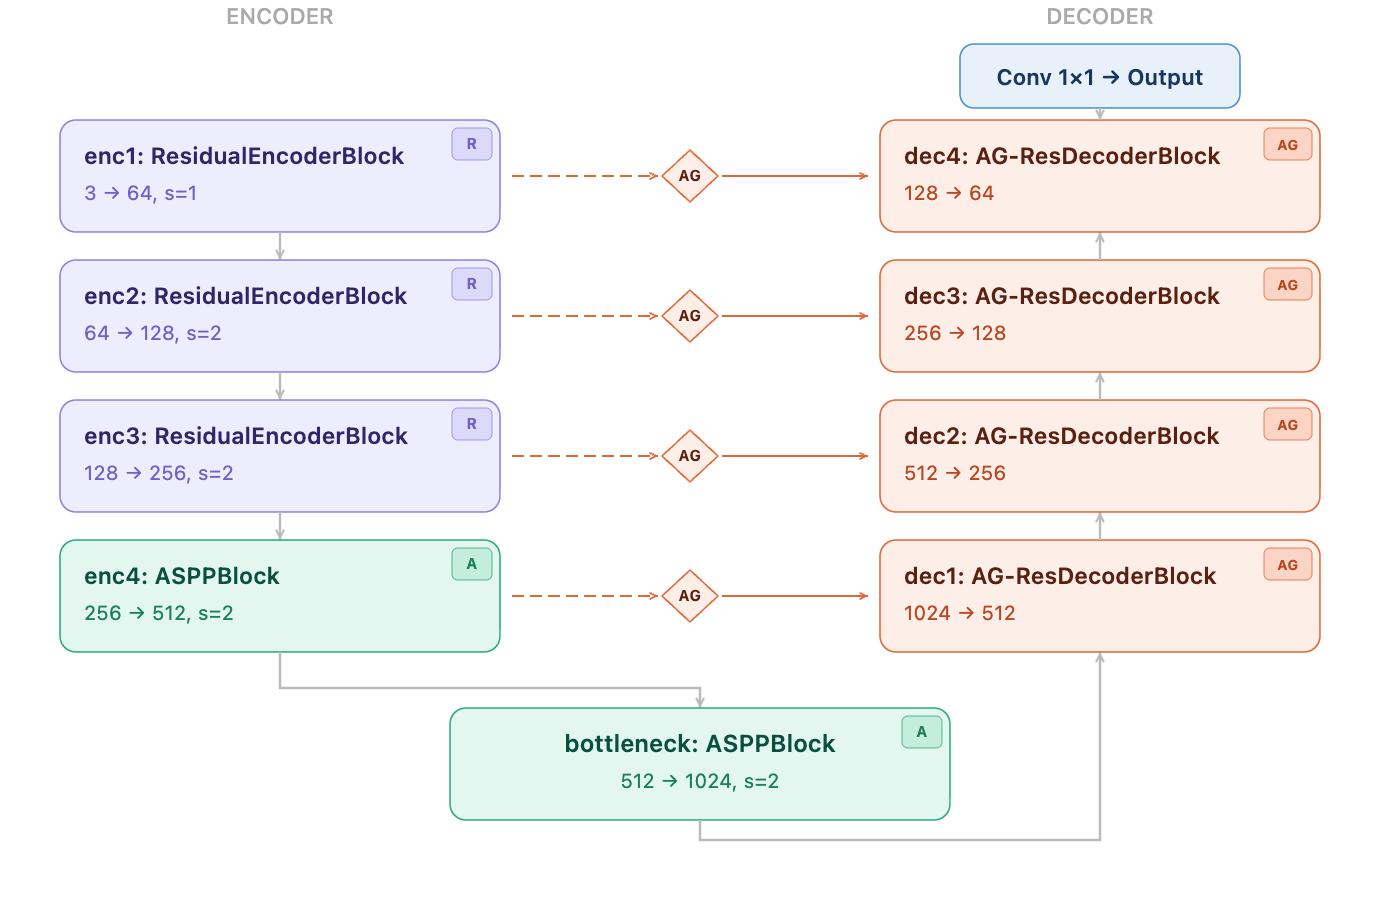
\includegraphics[width=\columnwidth]{architecture.png}
\caption{AG-ASPP-ResU-Net backbone. Residual encoder blocks
(\texttt{R}) in the early stages, an ASPP block (\texttt{A}) at the
last encoder stage and the bottleneck, and attention-gated decoder
blocks (\texttt{AG}) that selectively fuse encoder skips. U-Net,
ResU-Net, and ASPP-ResU-Net share the same U-shape but progressively
drop the \texttt{AG}, \texttt{ASPP}, and residual components
respectively.}
\label{fig:deep_arch}
\end{figure}

\begin{figure}[!htbp]
\centering
\setlength{\abovecaptionskip}{4pt}
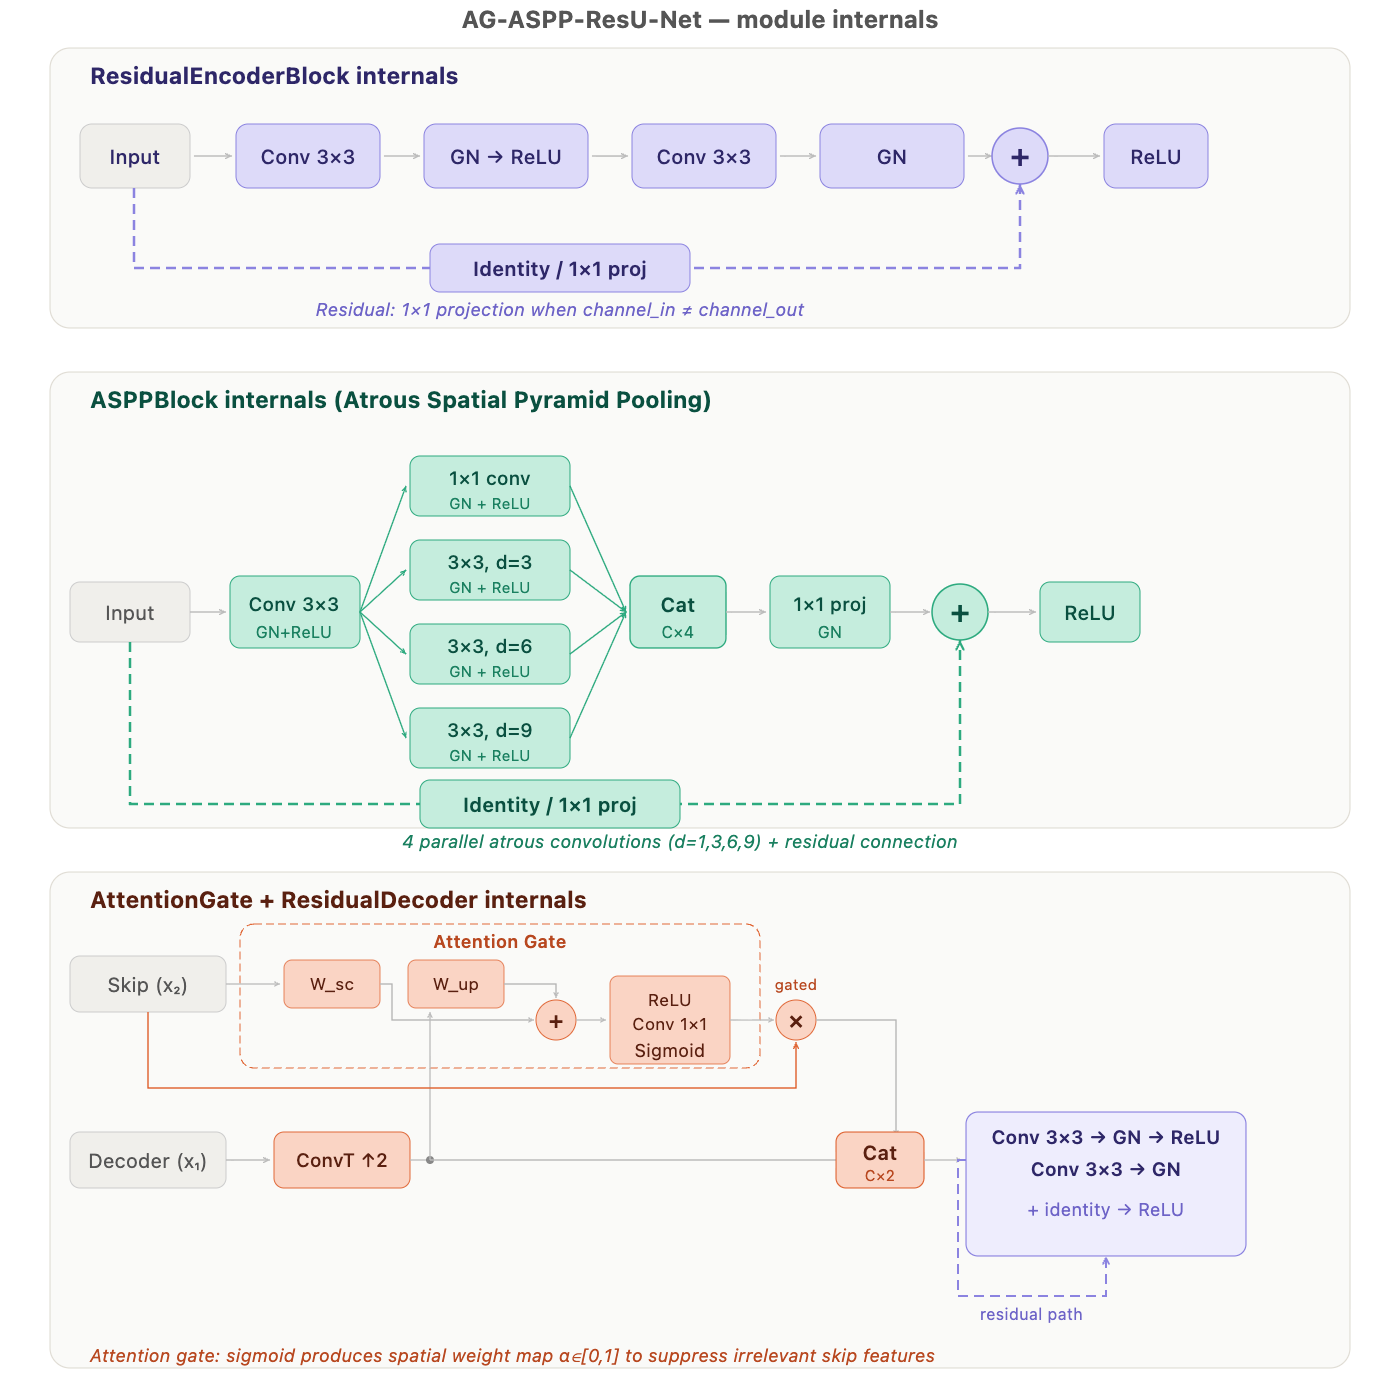
\includegraphics[width=\columnwidth]{modules.png}
\caption{Internals of the three distinguishing blocks in
AG-ASPP-ResU-Net. Top: residual encoder block (two-conv stack with
GroupNorm and $1{\times}1$ identity projection). Middle: ASPP block
(four parallel atrous convolutions at dilations $\{1,3,6,9\}$ fused by
concatenation and a $1{\times}1$ projection, plus an identity
residual). Bottom: attention-gated residual decoder (skip feature $x_2$
gated by a sigmoid map $\alpha\in[0,1]$ computed from projected skip
and upsampled decoder features, then concatenated with the upsampled
decoder feature $x_1$ and passed through a residual conv block).}
\label{fig:deep_modules}
\end{figure}

\subsection{Training Configuration and Implementation Choices}

All deep models are trained under the same protocol so that differences
in performance can be attributed to architecture rather than
inconsistent optimization. Input images are normalized to $[0, 1]$, and
the segmentation masks are converted into binary form with plant pixels
treated as the positive class.

The loss function combines \textbf{binary cross-entropy with logits}
and \textbf{Dice loss}~\cite{milletari2016} in equal proportion. This choice reflects the
fact that the task requires both stable pixel-wise learning and strong
overlap quality between prediction and ground truth. Binary
cross-entropy supports optimization at the pixel level, while Dice loss
directly emphasizes region-level agreement, which is particularly useful
in segmentation settings with foreground-background imbalance.

Optimization is carried out using \textbf{AdamW}~\cite{loshchilov2019}
with an initial
learning rate of $1 \times 10^{-4}$. Learning rate reduction on
validation plateau and early stopping are both applied so that the
comparison reflects the best achievable model state rather than
arbitrary final-epoch behaviour. In the main architecture comparison,
the batch size is set to 3, the maximum number of epochs is 100, and
the inference threshold is 0.6. A fixed random seed of 42 is used
throughout the experiments. During training, checkpoints are saved and
the best-performing checkpoint on validation loss is used for final
evaluation.

The framework also supports feature-augmented inputs, including ExG and
HSV-derived channels. These are introduced only in ablation experiments,
allowing the study to test whether explicit agricultural priors still
provide useful information once the model is already able to learn
hierarchical representations directly from RGB input.

\subsection{Evaluation Design and Robustness Protocol}

Our evaluation is designed to do more than identify the highest
clean-set score. All methods are first tested on the standard
train/validation/test split, using the same preprocessing pipeline and
the same resized image resolution. Performance is measured with
class-wise IoU, precision, recall, F1-score, overall accuracy,
confusion matrices, and inference time.

A second part of the evaluation focuses on robustness. Since field
imagery is rarely collected under ideal conditions, the models are
further tested under several controlled corruption types:
\textbf{Gaussian noise}, \textbf{Gaussian blur}, \textbf{brightness
shift}, \textbf{affine rotation}, and \textbf{JPEG compression}. Each
corruption is applied at multiple severity levels so that degradation
trends can be observed rather than inferred from a single perturbed
setting.

This robustness-oriented design is central to the study. It allows the
comparison to distinguish between models that perform well only under
clean benchmark conditions and models that remain reliable when image
quality changes. In this way, the evaluation framework supports a more
practical interpretation of segmentation performance, one that is closer
to real deployment conditions in agricultural environments.

\section{Experimental Results}

\subsection{Evaluation Protocol}

All methods were evaluated under the same train/validation/test split
and preprocessing pipeline described in Section~III. We
report class-wise IoU and F1-score, pixel accuracy, confusion matrices,
and inference time. To examine reliability beyond the clean setting,
robustness was further evaluated under controlled corruptions, including
Gaussian noise, Gaussian blur, brightness shift, affine rotation, and
JPEG compression, each tested at multiple severity levels. Gaussian
noise was evaluated at five severity levels, with the highest level
corresponding to variance 0.2.

\subsection{Traditional Segmentation Methods}

The traditional segmentation results show a clear and somewhat
counterintuitive pattern: the simplest colour-based approaches
outperform more elaborate region-based and probabilistic methods by a
substantial margin. ExG achieves the strongest result in this group,
with a Plant IoU of 0.754 and pixel accuracy of 0.903---numbers that
already approach the classical machine learning baselines. HSV
thresholding is the next strongest, with Plant IoU 0.708 and accuracy
0.897. Both methods require no training data and run in under 25\,ms
per image.

The more complex traditional methods do not improve on these simple
baselines. DenseCRF, which refines ExG predictions with bilateral and
Gaussian pairwise potentials, reaches Plant IoU 0.544---below ExG
despite taking 3.1\,s per image. GrabCut and Watershed produce weaker
results still (Plant IoU 0.499 and 0.376 respectively). Watershed's
low Soil IoU (0.211) reflects a structural limitation: when the soil
region does not contain enough pixels with strongly negative ExG to
seed definite-soil markers, Watershed floods large soil areas into the
plant label. K-means and edge-based segmentation perform weakest,
with Plant IoU below 0.30, confirming that unsupervised colour grouping
and low-level gradient detection alone are insufficient for this task.

Table~\ref{tab:trad} summarises all traditional method results.
Figure~\ref{fig:trad_comparison} compares them visually.

\begin{table}[t]
\centering
\caption{Test-set performance of traditional segmentation methods.}
\label{tab:trad}
\renewcommand{\arraystretch}{1.1}
\setlength{\tabcolsep}{3.5pt}
\begin{tabular}{@{}lcccc@{}}
\toprule
\textbf{Method} & \textbf{Acc.} & \textbf{Plant IoU} & \textbf{Plant F1} & \textbf{Time (s)} \\
\midrule
ExG              & 0.9032 & 0.7536 & 0.8595 & 0.025 \\
HSV thresholding & 0.8972 & 0.7083 & 0.8292 & 0.011 \\
DenseCRF         & 0.7494 & 0.5444 & 0.7050 & 3.114 \\
GrabCut          & 0.6814 & 0.4992 & 0.6659 & 4.146 \\
Watershed        & 0.4650 & 0.3758 & 0.5463 & 0.062 \\
K-means          & 0.5831 & 0.2967 & 0.4576 & 1.560 \\
Edge-based       & 0.5796 & 0.2614 & 0.4145 & 0.036 \\
\bottomrule
\end{tabular}
\end{table}

\begin{figure}[!htbp]
\centering
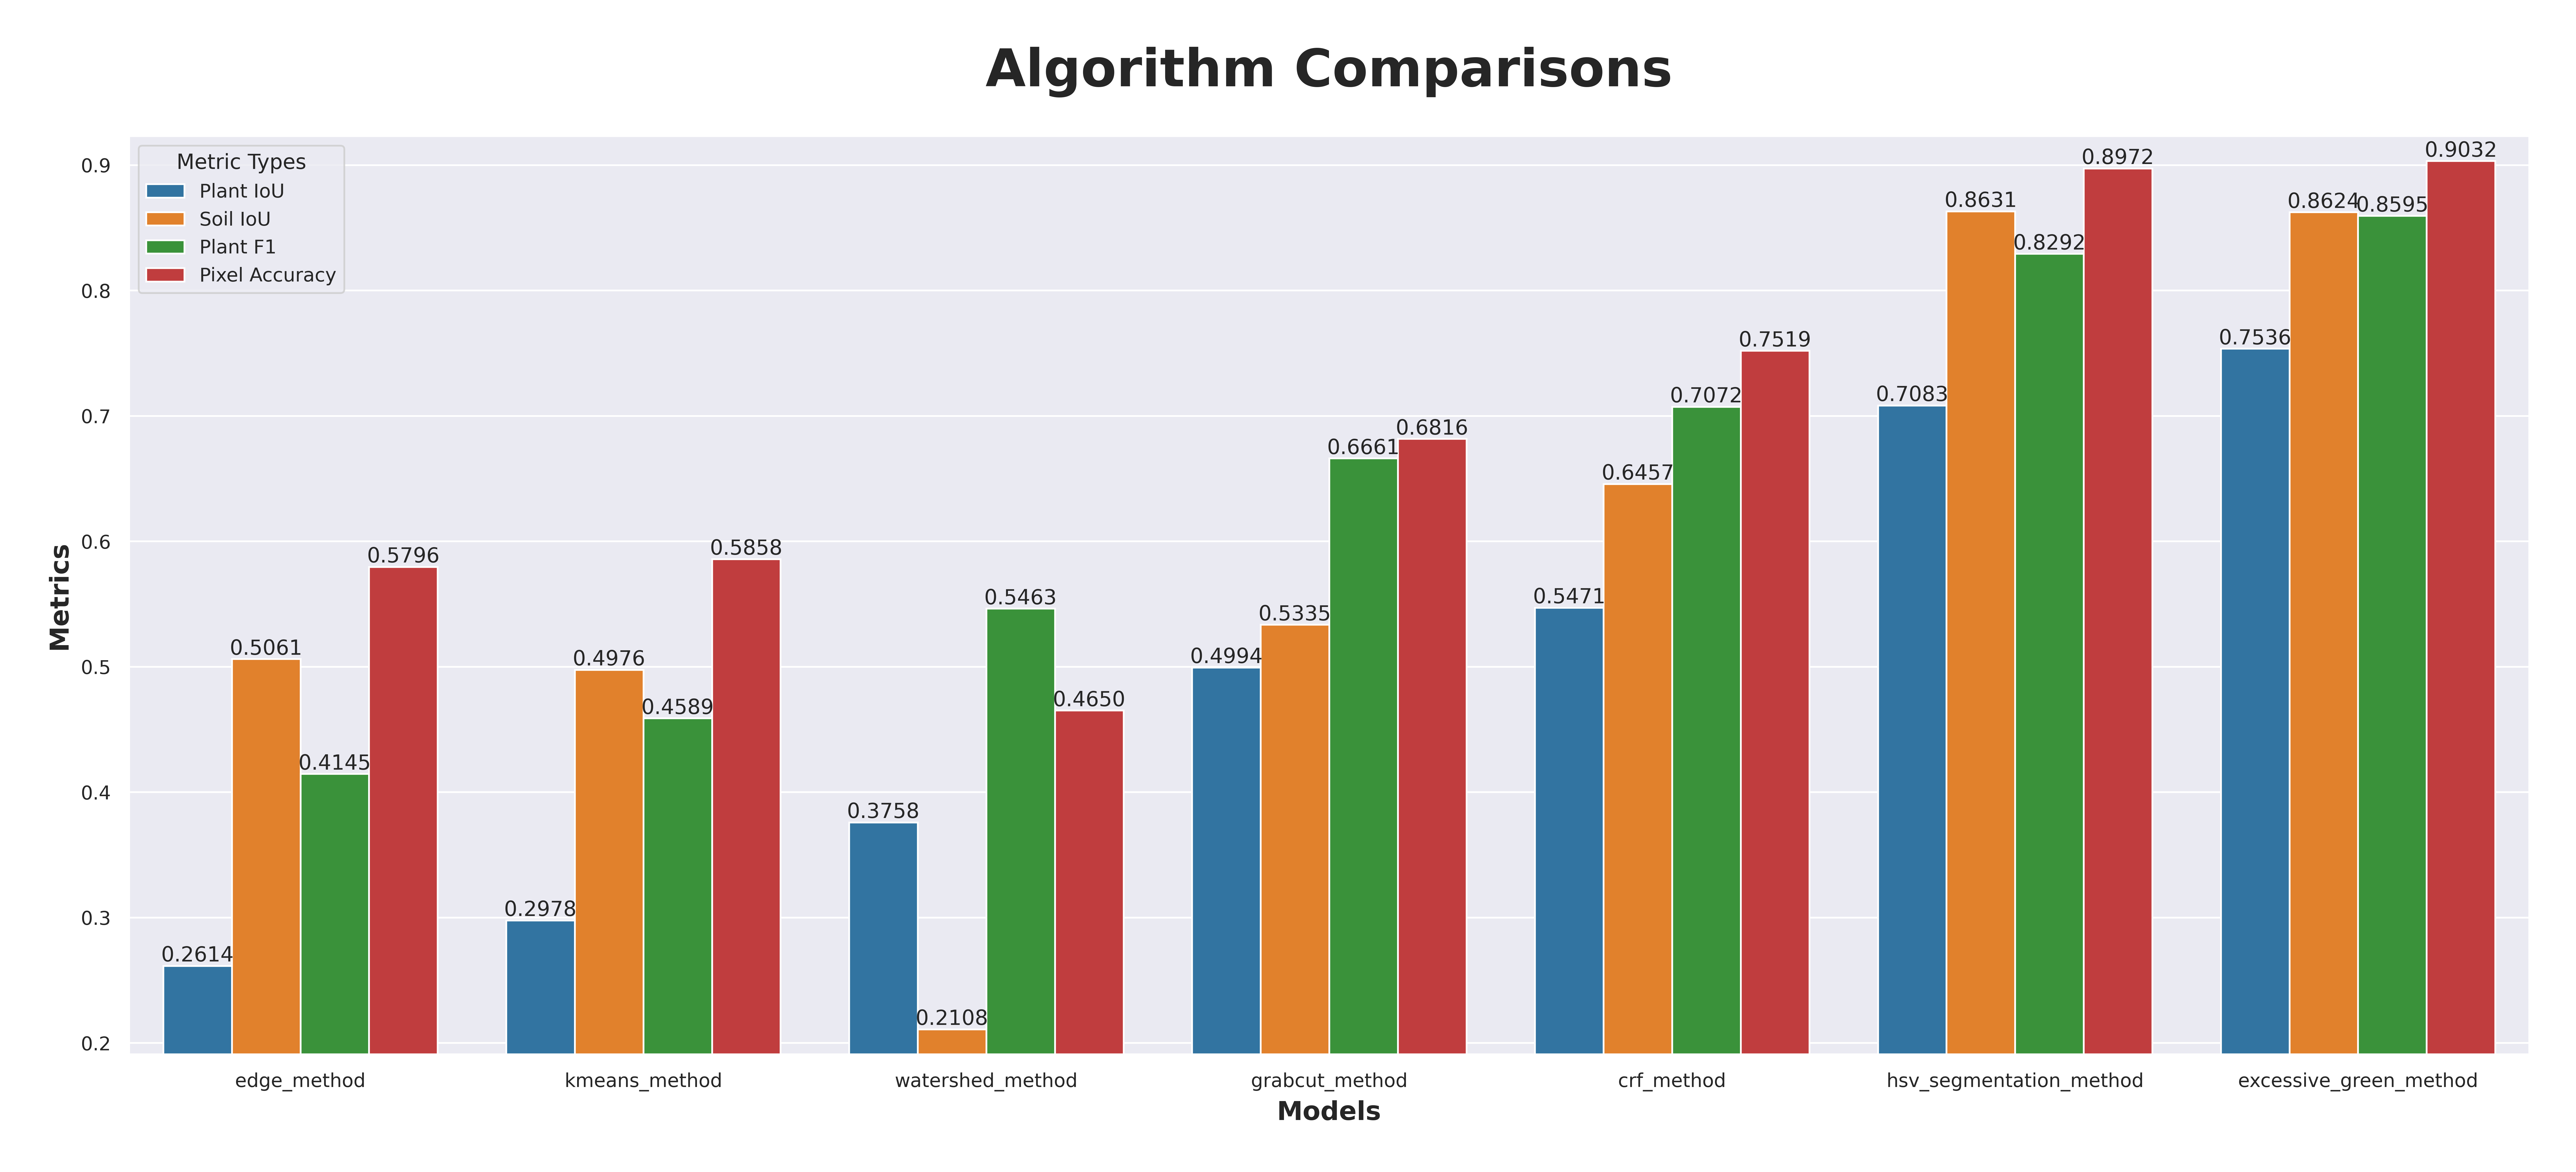
\includegraphics[width=\columnwidth]{comparisons/classic_cv_comparisons.png}
\caption{Comparison of traditional segmentation methods on the test
set. ExG and HSV thresholding achieve the strongest results despite
requiring no training, while more complex methods such as DenseCRF
and GrabCut underperform at substantially higher inference cost.}
\label{fig:trad_comparison}
\end{figure}

\subsection{Classical ML Baselines and Feature Effects}

The classical results already show a clear pattern. Plant-soil
separation can be achieved to a reasonable extent using handcrafted
colour information, but the quality remains limited once the visual
conditions become less ideal. Both Logistic Regression and Random Forest
improve when moving beyond RGB-only features, and the gain from adding
HSV is especially clear. However, the extra ExG channel brings only a
small improvement, particularly for Logistic Regression. This suggests
that explicit feature engineering is useful, but only up to a point.

\begin{table}[t]
\centering
\caption{Test-set performance of classical methods under different
feature configurations.}
\label{tab:classical}
\renewcommand{\arraystretch}{1.1}
\setlength{\tabcolsep}{3pt}
\begin{tabular}{@{}llcccc@{}}
\toprule
\textbf{Method} & \textbf{Feature set} & \textbf{Acc.} &
  \textbf{Plant IoU} & \textbf{Plant F1} & \textbf{Time (s)} \\
\midrule
Logistic Reg. & RGB         & 0.8689 & 0.7016 & 0.8247 & 0.048 \\
Logistic Reg. & RGB+HSV     & 0.8774 & 0.7130 & 0.8325 & 0.098 \\
Logistic Reg. & RGB+HSV+ExG & 0.8774 & 0.7130 & 0.8325 & 0.104 \\
\midrule
Random Forest & RGB         & 0.8575 & 0.6665 & 0.7999 & 1.187 \\
Random Forest & RGB+HSV     & 0.8597 & 0.6786 & 0.8085 & 1.144 \\
Random Forest & RGB+HSV+ExG & 0.8676 & 0.6902 & 0.8167 & 1.136 \\
\bottomrule
\end{tabular}
\end{table}

These results confirm that handcrafted features remain useful when the
model itself is relatively simple. At the same time, they also show the
ceiling of that approach. Even the best classical configuration still
falls well short of the deep models, which suggests that the main
challenge in this task is not only learning better colour thresholds,
but also learning spatial structure more effectively. ExG is therefore
best understood as a strong zero-training baseline rather than a
competitive alternative to the deep models.

\begin{figure}[!htbp]
\centering
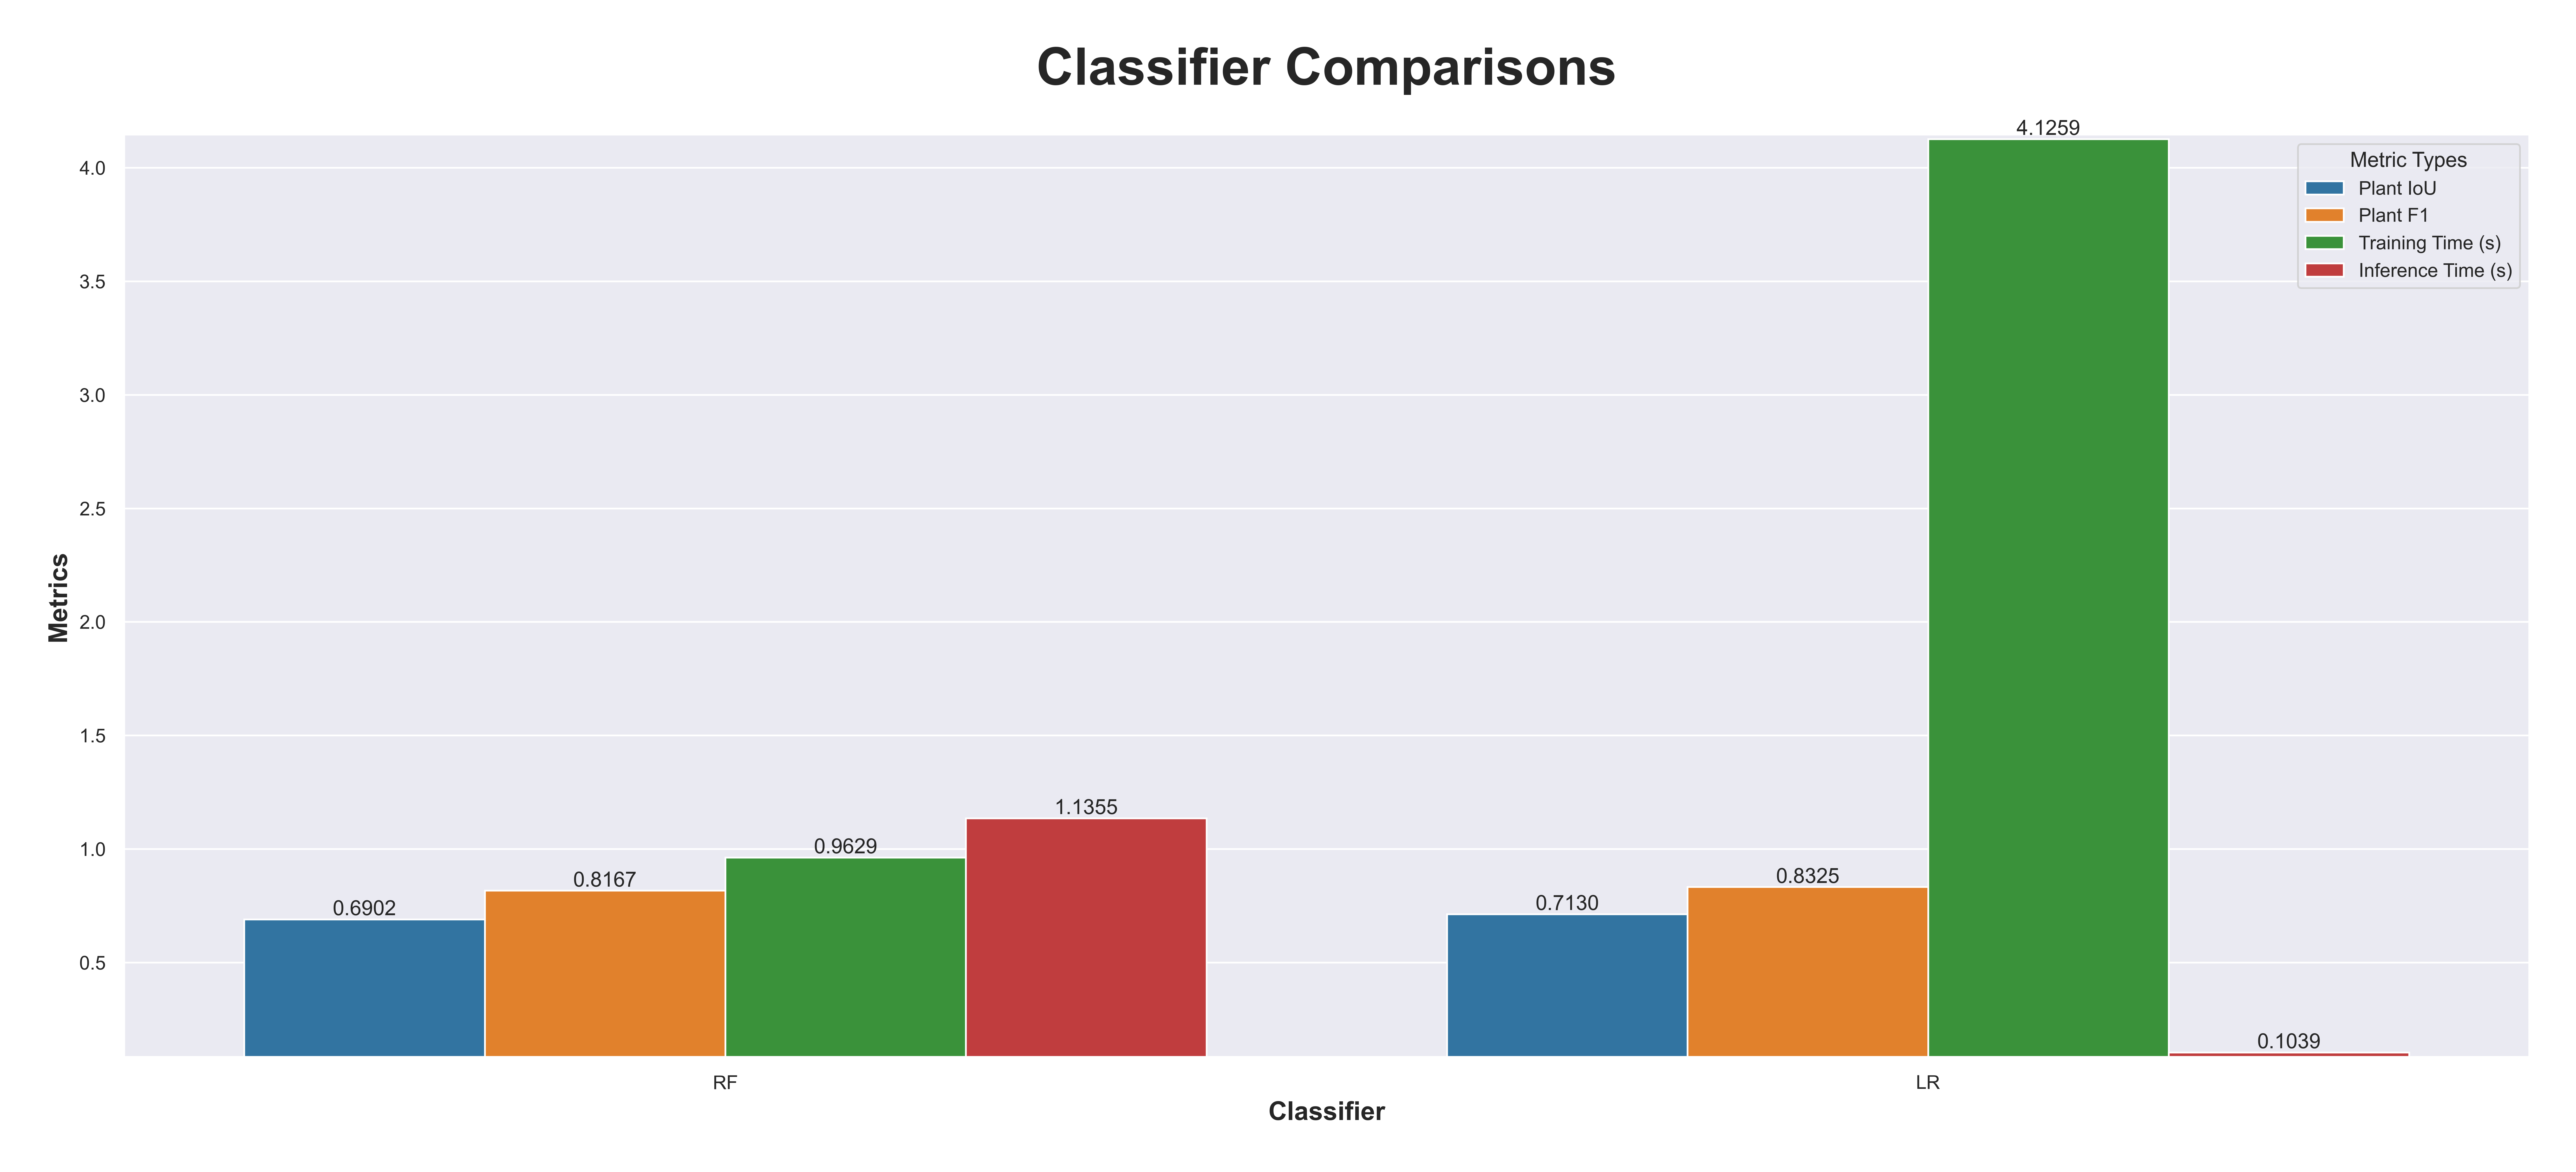
\includegraphics[width=\columnwidth]{comparisons/classifier_comparison.png}
\\[2pt]
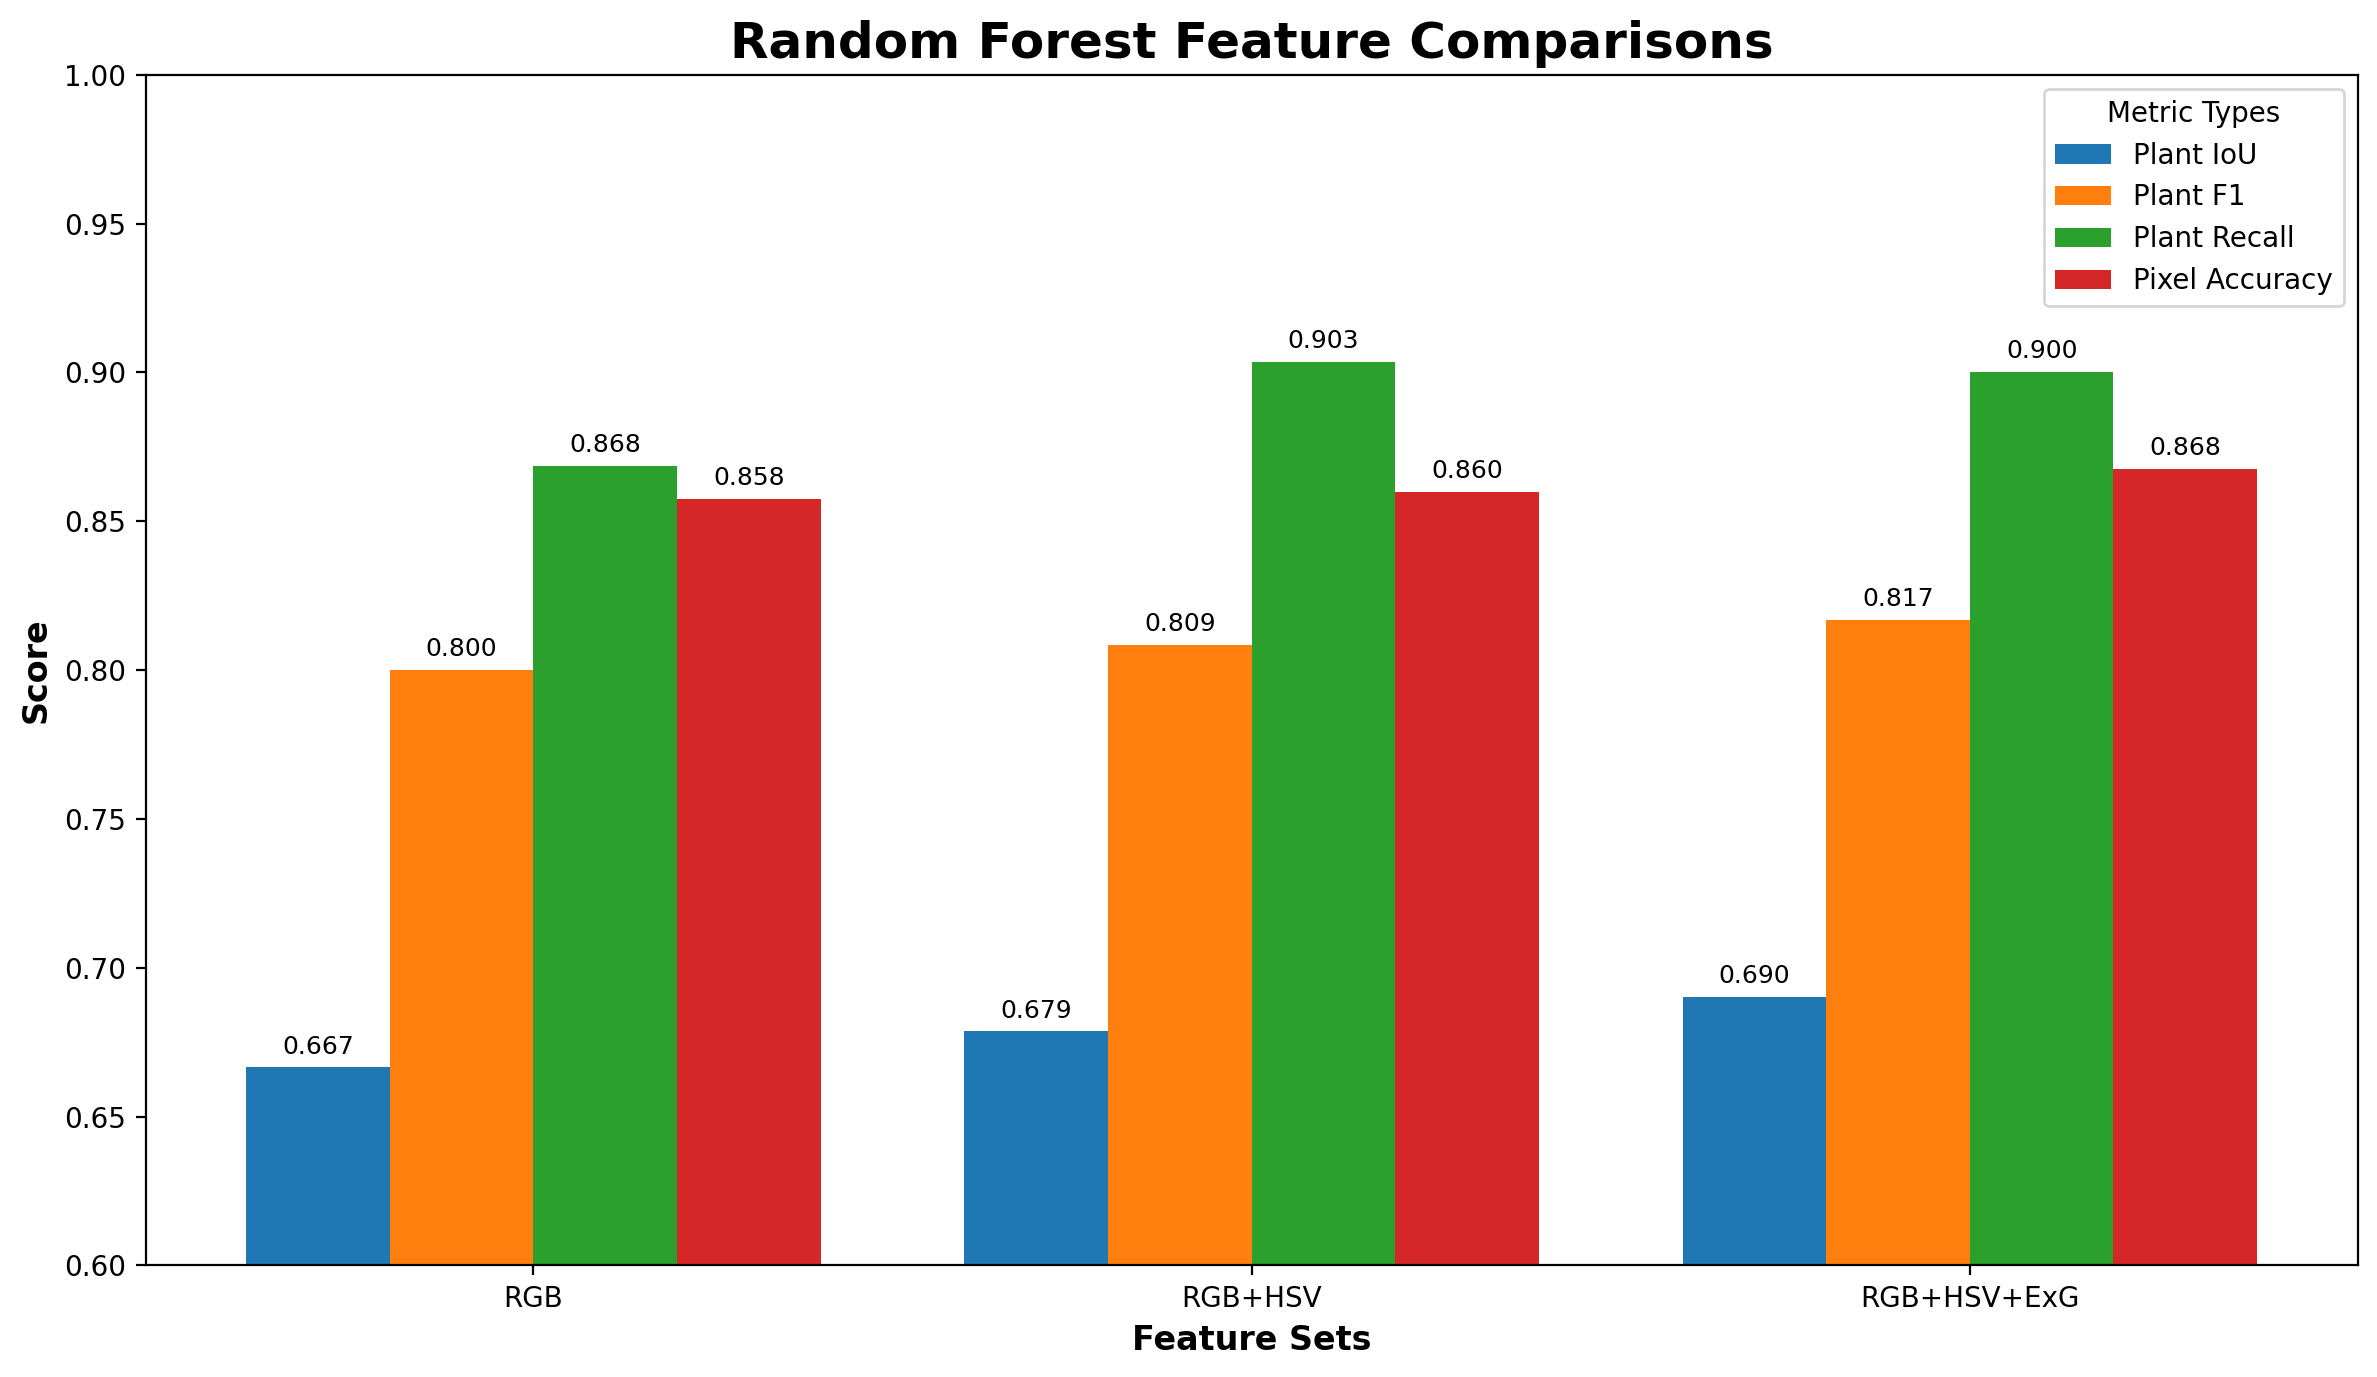
\includegraphics[width=\columnwidth]{comparisons/rf_feature_comparison.png}
\caption{Classical ML baselines. Top: Logistic Regression vs.\
Random Forest on Plant IoU/F1 and time. Bottom: Random Forest feature
ablation---RGB$\to$RGB+HSV gives the clearest gain, while adding ExG
yields only a small further improvement.}
\label{fig:classical_comparison}
\end{figure}

\subsection{Deep Model Comparison on Clean Splits}

The deep model results tell a more structured story than a simple
ranking of performance. All four encoder-decoder architectures clearly
outperform the classical baselines, and all of them surpass the best
Plant IoU of 0.775 reported in the original paper~\cite{zenkl2022},
with our strongest model reaching 0.8327---an improvement of 5.77
percentage points on this metric. The most important change within the
deep-model progression, however, happens early. Moving from U-Net to
ResU-Net produces the largest improvement, while ASPP and attention
gating provide smaller but still consistent refinements. The best
clean-set performance is achieved by Attention-Gated ASPP-ResU-Net,
although the gap between the top three deep models is relatively small
compared with the jump from U-Net to ResU-Net.

A closer comparison shows that the largest single gain came from moving
from U-Net to ResU-Net, with Plant IoU increasing by about 1.29
percentage points. By contrast, ASPP and attention gating produced
gains of 0.03 and 0.06 percentage points respectively. This suggests
that residual learning contributed more to final performance than later
architectural refinements. The improvement from ASPP was especially
limited, which is consistent with the nature of this task: in binary
plant-soil segmentation, the scale variation is narrower than in more
complex scene-segmentation problems, so the value of multi-scale
receptive fields may be less pronounced.

Attention gating did not change the ranking dramatically, but it appears
to have improved the balance between precision and recall on the plant
class, partly reducing the false-negative tendency seen in earlier
models. The validation scores are also consistently slightly higher than
the test scores. For the best model, the validation-test gap in Plant
IoU is about 1.2 percentage points. This gap is attributable to a
year-based distribution shift: the training and validation sets contain
images from 2018--2020, while the test set contains images from 2017,
where illumination and soil conditions differ. This is consistent with
the year variability analysis in the original paper~\cite{zenkl2022},
and reflects a stable domain shift rather than unstable training.

\begin{table*}[t]
\centering
\caption{Deep-model performance across train, validation, and test splits.}
\label{tab:deep}
\renewcommand{\arraystretch}{1.1}
\setlength{\tabcolsep}{5pt}
\begin{tabular}{@{}lccccccc@{}}
\toprule
\textbf{Model} &
  \textbf{Train Plant IoU} &
  \textbf{Val Plant IoU} &
  \textbf{Test Plant IoU} &
  \textbf{Test Plant F1} &
  \textbf{Test Soil IoU} &
  \textbf{Test Accuracy} &
  \textbf{Inference (s)} \\
\midrule
U-Net (Baseline)     & 0.7659 & 0.8317 & 0.8189 & 0.9005 & 0.9078 & 0.9349 & 1.0233 \\
ResU-Net             & 0.8362 & 0.8424 & 0.8318 & 0.9082 & \textbf{0.9157} & 0.9405 & 1.1439 \\
ASPP-ResU-Net        & 0.8390 & 0.8397 & 0.8321 & 0.9084 & 0.9155 & 0.9405 & 1.1977 \\
AG-ASPP-ResU-Net     & \textbf{0.8501} & \textbf{0.8447} & \textbf{0.8327} & \textbf{0.9087} & 0.9156 & \textbf{0.9406} & 1.3510 \\
\midrule
Original paper best~\cite{zenkl2022} & --- & --- & 0.7750 & 0.8630 & 0.8990 & 0.9450 & --- \\
\bottomrule
\end{tabular}
\end{table*}

\begin{figure}[!htbp]
\centering
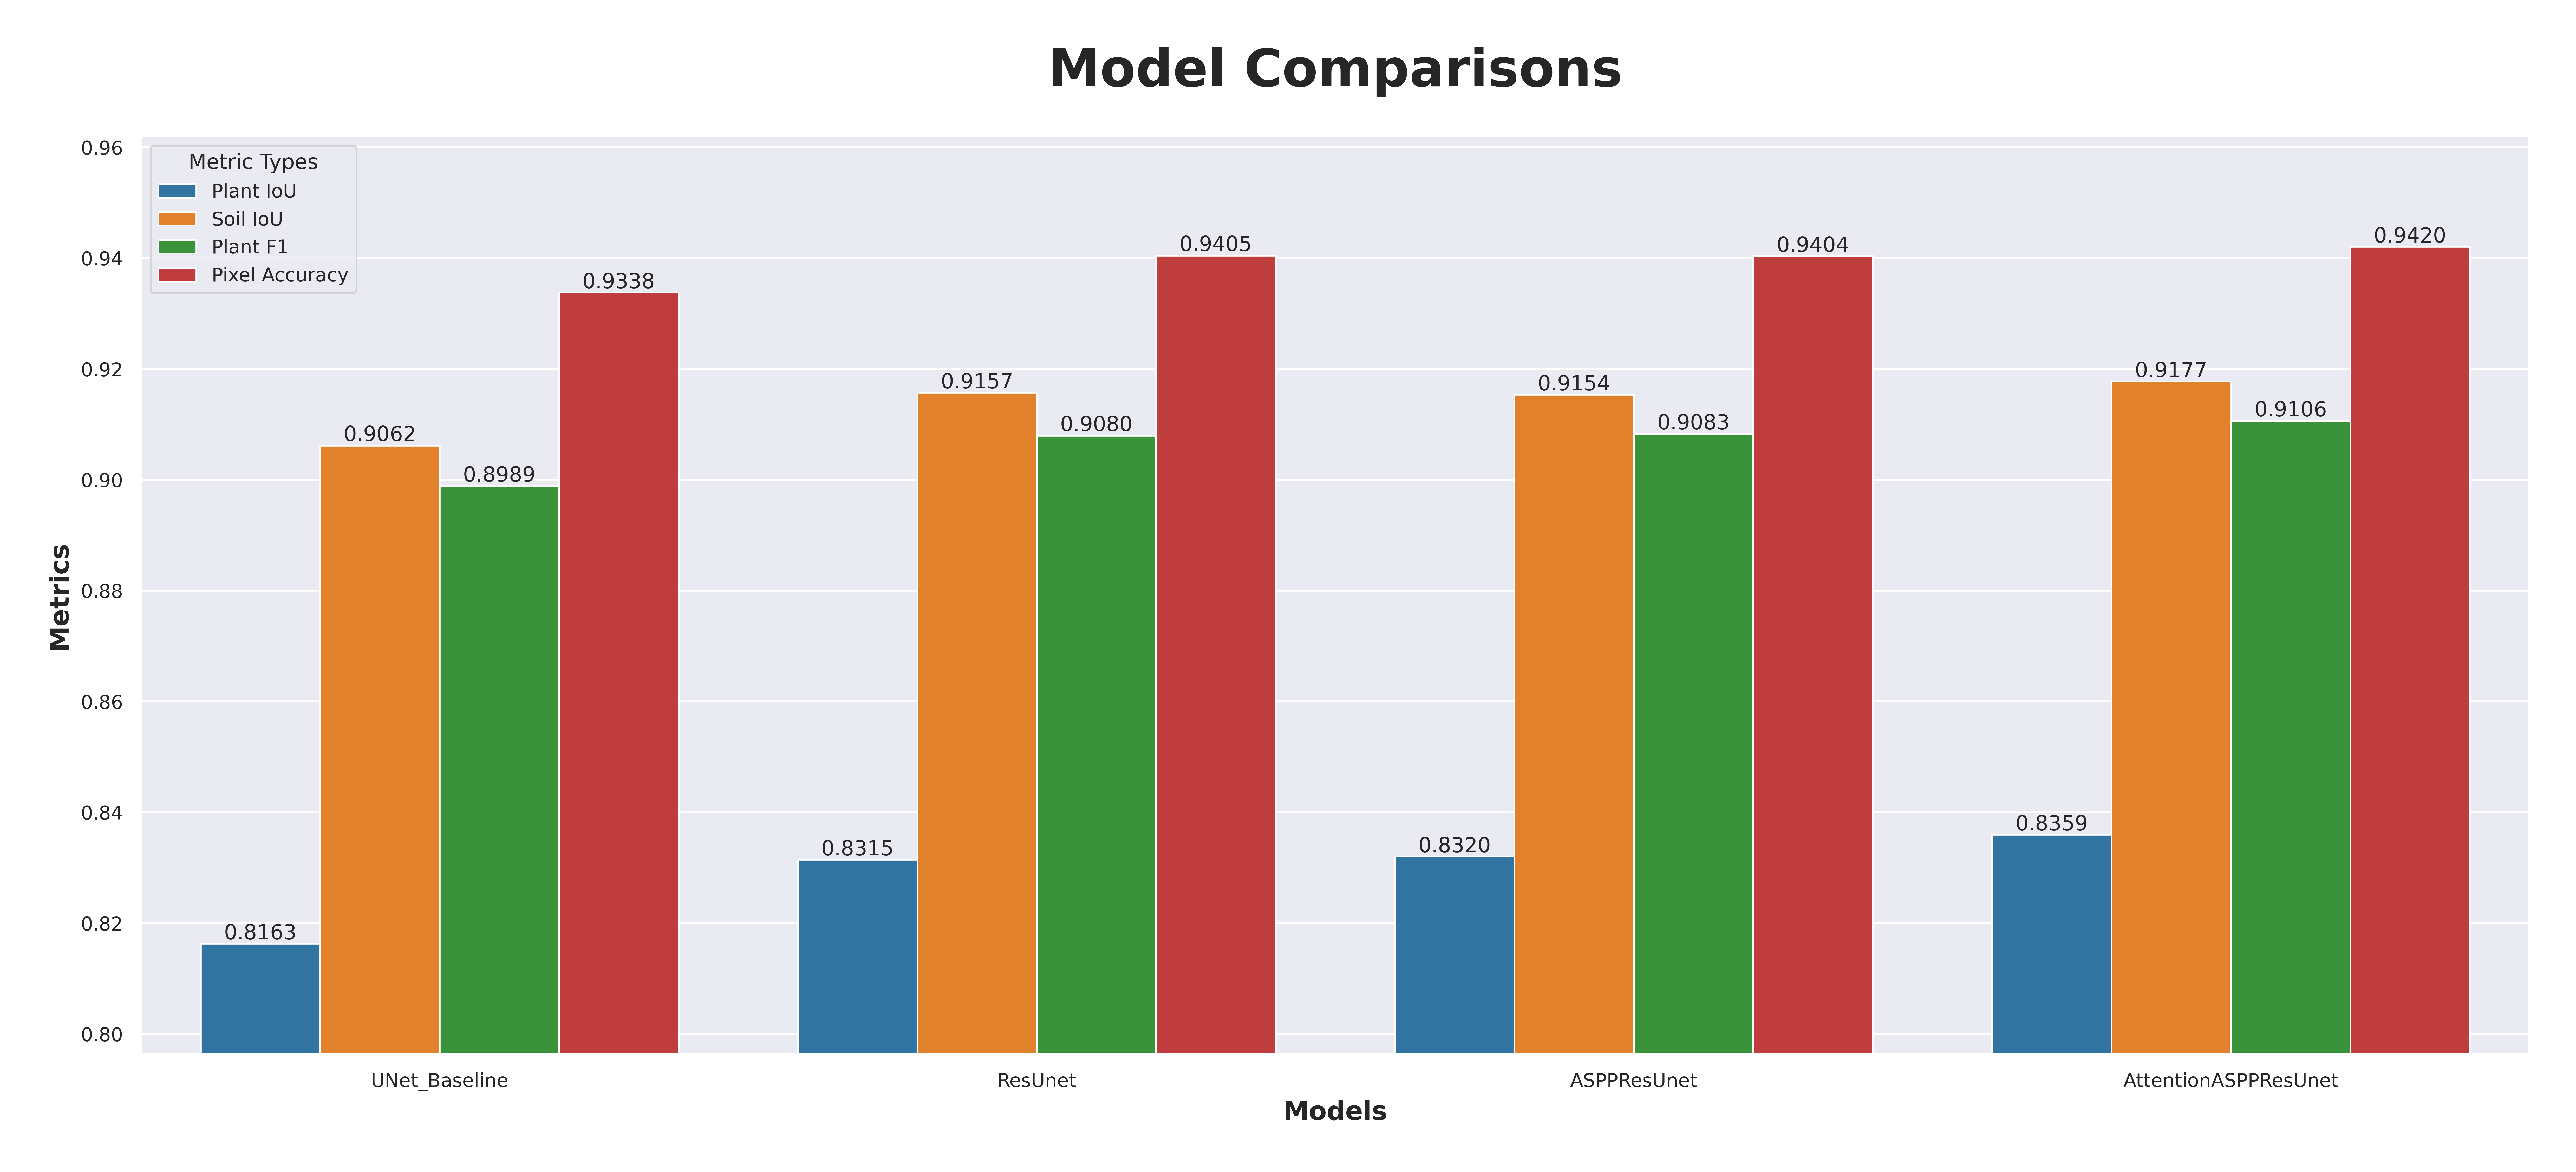
\includegraphics[width=\columnwidth]{comparisons/deep_learning_comparisons.png}
\caption{Test-set metrics across the four deep architectures. The
largest jump appears between U-Net and ResU-Net; ASPP and attention
gating deliver smaller additional gains.}
\label{fig:deep_comparison}
\end{figure}

\subsection{Training Behaviour and Confusion-Matrix Evidence}

The training curves show that all deep models converge in a stable way.
In later epochs, training loss continues to decrease while validation
loss tends to flatten or fluctuate slightly, which is consistent with
mild overfitting and supports the use of early stopping and
best-checkpoint selection. In our experiments, the best checkpoint often
appeared around epoch 40, after which training loss kept decreasing but
validation performance no longer improved. This pattern is typical of
small-dataset settings, where overfitting becomes visible before the
nominal end of training.

The confusion matrices tell a similar story from a different angle. The
strongest models separate the two classes reliably, but the remaining
mistakes are concentrated more on plant pixels than on soil pixels. This
suggests that the main difficulty is not general class confusion, but
more specific ambiguity around plant boundaries and weak foreground
structure (Fig.~\ref{fig:training_cm}).

\begin{figure}[!htbp]
\centering
\begin{minipage}{0.48\columnwidth}
\centering

\includegraphics[width=\linewidth]{AttentionASPPResUnet/plots/training_and_validation_loss_curves.png}
\end{minipage}\hfill
\begin{minipage}{0.48\columnwidth}
\centering

\includegraphics[width=\linewidth]{AttentionASPPResUnet/plots/confusion_matrix_test.png}
\end{minipage}
\caption{AG-ASPP-ResU-Net. Left: training and validation loss curves
showing stable convergence and a small late-epoch validation plateau.
Right: test-set confusion matrix---residual errors are concentrated on
plant pixels rather than soil, consistent with boundary-level ambiguity.}
\label{fig:training_cm}
\end{figure}

\subsection{Ablation and Negative Results}

The ablation experiments are useful because they show that not every
plausible modification leads to improvement. Adding ExG as an extra
deep-learning input sometimes makes early convergence slightly faster,
but it does not improve final segmentation quality. This is an
informative negative result, because ExG is highly relevant to
vegetation segmentation and might have been expected to help. Instead,
the result suggests that the convolutional models are already able to
learn similar colour-ratio cues directly from RGB input.

A learnable residual-scaling variant also underperforms the standard
residual design. With low alpha initialization, early gradients become
weaker and convergence slows down, leading to lower final performance
than the standard residual block.

\begin{table}[t]
\centering
\caption{Negative-result ablations.}
\label{tab:ablation}
\renewcommand{\arraystretch}{1.1}
\begin{tabular}{@{}p{1.9cm}p{3.0cm}l@{}}
\toprule
\textbf{Ablation} & \textbf{Main observation} & \textbf{Outcome} \\
\midrule
ExG concatenated into deep input &
  Slightly faster early convergence, but lower final quality than
  RGB-only baseline & Not adopted \\
\addlinespace
Learnable residual scaling ($\alpha$) &
  Slower optimization and lower final performance than standard
  residual block & Not adopted \\
\bottomrule
\end{tabular}
\end{table}

The learnable-residual variant reached a test Plant IoU of
about 0.8188, clearly below the standard ResU-Net result (0.8318).
These negative results matter because they clarify what the final gains
are \emph{not} coming from. In both cases, adding more structure or
more prior information did not help. This reinforces the idea that the
strongest improvements in this task come from effective feature
propagation rather than simply introducing more components.

\subsection{Robustness Analysis}

The robustness experiments reveal a fundamentally different picture from
the clean-set ranking, and contain the most practically significant
finding of the study.

Under affine rotation, performance remains very stable across all
models, with almost no significant drop across levels. Under Gaussian
blur, segmentation degrades moderately: for AG-ASPP-ResU-Net, Plant IoU
falls from 0.831 to 0.791 at the highest severity, a decline that
leaves the model still functional. JPEG compression shows a steeper
trend, with Plant IoU dropping from 0.810 to 0.620, indicating that
high-frequency boundary information matters more than it might appear.
Brightness shift shows an asymmetric pattern: underexposure causes
substantially more degradation than overexposure, and the resulting
curve is non-monotonic, suggesting that the models are more sensitive to
the loss of visible structure than to moderate saturation.

Gaussian noise, however, produces a qualitatively different and more
severe failure. At level 5 (variance 0.2), AG-ASPP-ResU-Net Plant IoU
drops to 0.005---a near-complete collapse. More importantly, this
vulnerability reveals a \textbf{ranking reversal} relative to clean-set
performance. Between noise levels 2 and 3, ResU-Net Plant IoU falls
sharply from 0.557 to 0.112; by noise level 5, all three residual-based
models collapse to essentially zero Plant IoU (ResU-Net 0.003,
ASPP-ResU-Net 0.005, AG-ASPP-ResU-Net 0.005). The plain U-Net, by
contrast, degrades much more gracefully and retains a Plant IoU of
0.271 at the same severity. On highly noisy inputs, the clean-set
ranking is therefore fully inverted: the model with the worst clean-set
performance outperforms every model that surpassed it under ideal
conditions (Fig.~\ref{fig:noise_reversal}).

\begin{figure}[!htbp]
\centering
\begin{minipage}{0.48\columnwidth}
\centering

\includegraphics[width=\linewidth]{UNet_Baseline/plots/robustness/gaussian_noise/robustness_iou_test.png}
\\ \small (a) U-Net
\end{minipage}\hfill
\begin{minipage}{0.48\columnwidth}
\centering

\includegraphics[width=\linewidth]{AttentionASPPResUnet/plots/robustness/gaussian_noise/robustness_iou_test.png}
\\ \small (b) AG-ASPP-ResU-Net
\end{minipage}
\caption{Ranking reversal under Gaussian noise. Plant/Soil IoU
vs.\ severity level. The plain U-Net degrades gradually (Plant IoU
0.735$\to$0.271), while AG-ASPP-ResU-Net collapses between levels~2
and~3, reaching 0.005 at level~5 despite leading on clean data.}
\label{fig:noise_reversal}
\end{figure}

\begin{table}[t]
\centering
\caption{Summary of robustness behaviour under different corruptions
(AG-ASPP-ResU-Net; noise comparison includes U-Net).}
\label{tab:robust}
\renewcommand{\arraystretch}{1.15}
\setlength{\tabcolsep}{3pt}
\begin{tabular}{@{}lp{1.4cm}p{3.2cm}@{}}
\toprule
\textbf{Corruption} & \textbf{Robustness} & \textbf{Key observation} \\
\midrule
Affine rotation  & Very strong & Almost no drop across levels \\
Gaussian blur    & Strong      & Plant IoU 0.831$\to$0.791 at highest severity \\
JPEG compression & Medium      & Plant IoU 0.810$\to$0.620; gradual boundary loss \\
Brightness shift & Uneven      & Underexposure $\gg$ overexposure; non-monotonic \\
Gaussian noise   & Weak        & All residual models $\le$0.005 at level~5;
                                 U-Net retains 0.271 (ranking reversed) \\
\bottomrule
\end{tabular}
\end{table}

\subsection{Failure Cases and Overall Findings}

The failure cases bring the quantitative results into focus
(Fig.~\ref{fig:failure}). The hardest examples usually involve
low-contrast plant boundaries, dark illumination, or severe image
degradation. These are not isolated mistakes, but recurring patterns
that match the corruption experiments and confusion-matrix trends.

\begin{figure}[!htbp]
\centering
\begin{minipage}{0.48\columnwidth}
\centering

\includegraphics[width=\linewidth]{AttentionASPPResUnet/failures/test/ground_truth_0.png}
\\ \small (a) Ground truth
\end{minipage}\hfill
\begin{minipage}{0.48\columnwidth}
\centering

\includegraphics[width=\linewidth]{AttentionASPPResUnet/failures/test/predicted_0.png}
\\ \small (b) Prediction
\end{minipage}
\caption{Representative failure case (AG-ASPP-ResU-Net, test split).
Thin low-contrast plant structures are under-segmented, producing
fragmented predictions relative to the ground-truth mask.}
\label{fig:failure}
\end{figure}

In total, the results reveal a consistent pattern. Classical methods
remain useful as efficient references, but their dependence on
handcrafted features limits their ceiling. Deep learning models are
substantially stronger, and all deep models exceed the original paper
benchmark. Most of the meaningful clean-set gain comes from better
optimization and feature propagation rather than from simply increasing
complexity. Attention-Gated ASPP-ResU-Net gives the best clean-set
result, but the robustness experiments reveal a serious weakness: the
residual-based designs that improve clean-set learning are also
associated with substantially weaker robustness under severe Gaussian
noise, producing a ranking reversal that has direct implications for
real-world deployment.

\section{Discussion}

A clear pattern still emerges from the results. On the clean test set,
the strongest overall performance still comes from the deep
encoder-decoder models, and the most important gain within that group
appears in the transition from U-Net to ResU-Net. This indicates that,
in our setting, better optimization and feature propagation matter more
than simply adding extra modules. ASPP and attention gating still
provide useful refinements, but their contributions are much smaller
than the gain introduced by residual learning.

The comparison with non-deep methods helps clarify that bottleneck.
Among the traditional segmentation methods, the strongest results come
from the simplest colour-based approaches: ExG (Plant IoU 0.754) and
HSV thresholding (0.708). More elaborate alternatives such as DenseCRF,
GrabCut, and Watershed all perform worse despite higher computational
cost, which shows that procedural complexity does not automatically
translate into better segmentation in a fully automatic setting. One
clear reason is that the more complex methods still depend on the same
colour prior (ExG) for initialisation; when that prior is imperfect,
the refinement steps cannot fully recover. The failure of Watershed to
achieve adequate Soil IoU---because insufficient soil-seed pixels are
found in some images---illustrates this dependency directly.

ExG, HSV thresholding, Logistic Regression, and Random Forest all
remain meaningful baselines because they are fast, interpretable, and
grounded in useful colour information. At the same time, their
performance clearly plateaus below that of the encoder-decoder models.
This suggests that the main advantage of the deep models is not just
better colour discrimination, but the ability to use spatial structure,
local texture, and boundary information in a more coherent way.

The negative results reinforce this interpretation. ExG concatenation
into the deep models is a particularly informative failure case:
although ExG is a highly relevant vegetation prior, adding it as an
extra input channel does not improve final deep-model performance. This
suggests that the convolutional backbone already learns similar
colour-ratio cues directly from RGB data, consistent with the finding in
the original paper~\cite{zenkl2022}. A similar pattern appears in the
learnable residual-scaling variant, which adds parameterization but does
not outperform the standard residual design. Together, these failed
modifications indicate that the gains in this project do not come from
adding more information or more flexibility by default, but from changes
that improve how useful features are learned and propagated.

The robustness results add the most important qualification to the
clean-set narrative. The ranking reversal under strong Gaussian noise is
not a minor footnote: it reveals that the architectural change most
responsible for clean-set improvement---the residual shortcut---is
simultaneously associated with the greatest robustness failure. One
plausible explanation is that the additive nature of residual
connections allows noise injected at the input to propagate and
accumulate across successive blocks, whereas the plain encoder of U-Net
lacks this compounding path. GroupNorm, while effective for stabilizing
training on clean data, may be misled by noise-corrupted activation
statistics, potentially amplifying the problem at deeper layers. However,
these are observations and candidate mechanisms, not confirmed causal
claims: whether residual networks are categorically more or less
noise-robust than plain networks is known to be task- and
training-dependent, and targeted ablations would be required to isolate
the contribution of each component. What the data do establish
unambiguously is the ranking reversal itself, and its practical
consequence: under severe Gaussian noise, architectural sophistication
does not translate into robustness.

The validation-test gap is better understood as structural than
incidental. The 1.2 percentage-point drop in Plant IoU from validation
to test reflects a year-based distribution shift---training and
validation images were collected in 2018--2020, while test images are
from 2017---and is therefore an expected consequence of temporal domain
shift rather than a sign of unstable training.

In summary, the experiments suggest that the key challenge in this task
is not the absence of architectural complexity, but the difficulty of
learning representations that are both accurate on clean data and stable
under realistic corruption. Further progress is unlikely to come simply
from making the architecture more elaborate. More promising directions
include training strategies that target noise sensitivity directly, such
as noise-aware data augmentation, adversarial training, or architectural
choices that decouple feature propagation from noise accumulation.

\section{Conclusion}

Overall, the deep learning models remained the strongest, and all four
architectures surpassed the original paper benchmark of Plant IoU 0.775.
Within the deep-model comparison, the clearest clean-set improvement
came from moving from U-Net to ResU-Net, while later additions such as
ASPP and attention gating mainly provided smaller refinements.

The non-deep results were also informative. Among the traditional
segmentation methods, simple colour-based approaches such as ExG and
HSV thresholding performed better than more elaborate alternatives such
as Watershed and GrabCut. The machine learning baselines made more
flexible use of handcrafted features but still did not reach the level
of the deep models. Taken together, these comparisons show that colour
information remains highly useful in this task, but that stronger
segmentation ultimately depends on learning spatial structure more
effectively.

The negative results further clarified this picture. Neither ExG
concatenation nor learnable residual scaling improved final deep-model
performance, showing that not every plausible enhancement is useful once
the backbone is already strong. In this way, the study is not only about
ranking methods, but also about identifying which kinds of modifications
genuinely improve segmentation and which are largely redundant in this
setting.

The most important finding beyond the clean-set ranking is the
robustness reversal under severe Gaussian noise. All residual-based
models collapse sharply at high noise levels, while the plain U-Net
remains relatively more stable and retains a Plant IoU of 0.271 at the
highest severity. This reveals a clear accuracy-robustness trade-off in
the model designs used here, and has direct implications for real
agricultural deployment where image quality cannot always be guaranteed.

The main limitations of this study can already be seen in the result
patterns. The current setup is still mainly about plant-soil separation,
so the conclusions speak more directly to foreground-background
discrimination than to broader field understanding. The validation-test
gap also suggests that year-based domain shift is an important challenge
by itself, rather than just a small variation within the same setting.
Another issue is that all methods are evaluated at a fixed resized
resolution, which may remove some of the fine boundary detail needed for
thin leaves and weak foreground structures, where many of the remaining
errors are concentrated. More importantly, the results suggest that the
real bottleneck is no longer simply clean-set accuracy. The harder
problem is learning representations that remain reliable when the visual
cues become unstable. Future work should therefore focus less on adding
complexity for its own sake, and more on improving robustness to
temporal shift, boundary ambiguity, and other forms of visual
instability that are likely to matter in real field conditions.

\begin{thebibliography}{14}

\bibitem{ews}
ETH Research Collection, ``EWS-Dataset.''
[Online]. Available: \url{https://www.research-collection.ethz.ch/entities/researchdata/165d22fc-6b0f-4fc3-a441-20d8bdc50a70}

\bibitem{zenkl2022}
R.~Zenkl \emph{et al.}, ``Outdoor Plant Segmentation With Deep Learning for
High-Throughput Field Phenotyping on a Diverse Wheat Dataset,''
\emph{Frontiers in Plant Science}, vol.~12, p.~774068, 2022.

\bibitem{cao2025}
S.~Cao \emph{et al.}, ``The Blessing of Depth Anything: An Almost
Unsupervised Approach to Crop Segmentation with Depth-Informed Pseudo
Labeling,'' \emph{Plant Phenomics}, vol.~7, no.~1, p.~100005, 2025.

\bibitem{zhang2026}
J.~Zhang, S.~Cao, B.~Xu, Y.~Li, W.~Jia, T.~Wu, H.~Lu, W.~Hu, and
Z.~Han, ``DepthCropSeg++: Scaling a Crop Segmentation Foundation Model
With Depth-Labeled Data,'' \emph{IEEE J.~Sel.\ Topics Signal Process.},
vol.~20, pp.~129--141, 2026, doi: 10.1109/JSTSP.2026.3654362.

\bibitem{long2015}
J.~Long, E.~Shelhamer, and T.~Darrell, ``Fully Convolutional Networks for
Semantic Segmentation,'' in \emph{Proc.\ IEEE CVPR}, 2015, pp.~3431--3440.

\bibitem{woebbecke1995}
D.~M.~Woebbecke, G.~E.~Meyer, K.~Von~Bargen, and D.~A.~Mortensen,
``Color Indices for Weed Identification Under Various Soil, Residue, and
Lighting Conditions,'' \emph{Trans.\ ASAE}, vol.~38, no.~1, pp.~259--269,
1995.

\bibitem{hosmer2013}
D.~W.~Hosmer, S.~Lemeshow, and R.~X.~Sturdivant,
\emph{Applied Logistic Regression}, 3rd~ed.\ Hoboken, NJ: Wiley, 2013.

\bibitem{smith1978}
A.~R.~Smith, ``Color Gamut Transform Pairs,''
\emph{SIGGRAPH Comput.\ Graph.}, vol.~12, no.~3, pp.~12--19, 1978.

\bibitem{breiman2001}
L.~Breiman, ``Random Forests,'' \emph{Mach.\ Learn.},
vol.~45, no.~1, pp.~5--32, 2001.

\bibitem{ronneberger2015}
O.~Ronneberger, P.~Fischer, and T.~Brox, ``U-Net: Convolutional Networks
for Biomedical Image Segmentation,'' in \emph{Proc.\ MICCAI}, 2015,
pp.~234--241.

\bibitem{he2016}
K.~He, X.~Zhang, S.~Ren, and J.~Sun, ``Deep Residual Learning for Image
Recognition,'' in \emph{Proc.\ IEEE CVPR}, 2016, pp.~770--778.

\bibitem{chen2017}
L.-C.~Chen, G.~Papandreou, F.~Schroff, and H.~Adam, ``Rethinking Atrous
Convolution for Semantic Image Segmentation,'' \emph{arXiv:1706.05587},
2017.

\bibitem{oktay2018}
O.~Oktay \emph{et al.}, ``Attention U-Net: Learning Where to Look for the
Pancreas,'' \emph{arXiv:1804.03999}, 2018.

\bibitem{wu2018}
Y.~Wu and K.~He, ``Group Normalization,'' in \emph{Proc.\ ECCV}, 2018,
pp.~3--19.

\bibitem{loshchilov2019}
I.~Loshchilov and F.~Hutter, ``Decoupled Weight Decay Regularization,''
in \emph{Proc.\ Int.\ Conf.\ Learn.\ Represent.\ (ICLR)}, 2019.

\bibitem{milletari2016}
F.~Milletari, N.~Navab, and S.-A.~Ahmadi, ``V-Net: Fully Convolutional
Neural Networks for Volumetric Medical Image Segmentation,'' in
\emph{Proc.\ Int.\ Conf.\ 3D Vis.\ (3DV)}, 2016, pp.~565--571.

\end{thebibliography}

\end{document}